\chapter{Thickness One}

While results from the previous chapters resolve the question of $m(a_1,a_2,a_3,3)$ for $a_1 \geq a_2 \geq a_3 \geq 11$, similar constructions for smaller grids remain sparse. Nevertheless, computer examples seem to suggest that grids of minimum size at least 2 are largely optimal. Grids of thickness 1 tell a different story. In this chapter, we prove that the only perfect grids in thickness 1 are those of the form $[2^n-1]^2$. This answers a question posed by Benevides et al. in \cite{benevides}.

\section{A tight result for $[n]^2$}
The proof is structured as follows: Let $A_0$ be a perfect lethal set on the grid $(a_1, a_2, 1)$. We show that the structure of $A_0$ guarantees the existence of a perfect lethal set on the smaller grid $(\frac{a_1-1}{2}, \frac{a_1-1}{2}, 1)$. Repeated applications of this process of reduction guarantee the existence of a perfect lethal set on the grid $(a_0, 1,1)$. Since the only such grid that admits a perfect lethal set is $(1,1,1)$, we are forced to conclude that $a_1 = a_2 = 2^k-1$ for some $k > 0$. 

For the remainder of the chapter, let $G = [a_1] \times [a_2]$. Recall that perfect lethal sets match the surface area bound. In particular,
$$|A_0| = \frac{a_1a_2 + a_1 + a_2}{3}.$$
We begin with the following observations regarding the structure of $A_0$:

\begin{prop}
\label{prop:alternating_border}
If $A_0$ is a perfect lethal set on $G$, then $A_0$ contains alternating vertices along the border of $G$. 
\end{prop}

\begin{proof}
Since $A_0$ is perfect, it must form an independent set in $G$. By Proposition \ref{prop:border}, no two adjacent border vertices are both uninfected. Together, these conditions ensure that $A_0$ intersects the border of $G$ in an alternating pattern (see Figure \ref{fig:border}). 
\end{proof}

\begin{figure}[]
\centering
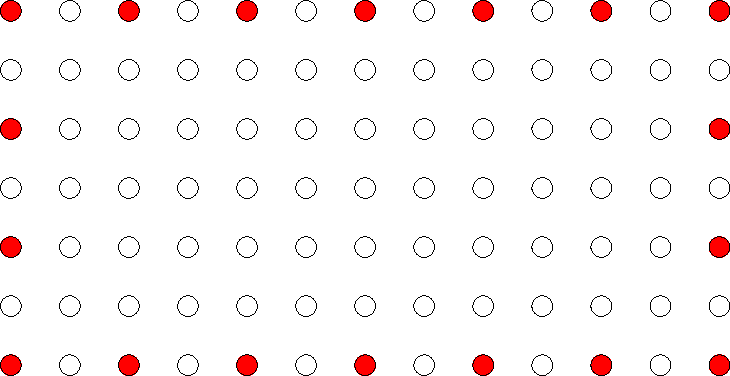
\includegraphics[width=0.5\textwidth]{figures/6/border.pdf}
\caption{Alternating infection along the border of $[7] \times [13]$.}
\label{fig:border}
\end{figure} 

\begin{prop}
If $A_0$ is a perfect lethal set on $G$, then $a_1, a_2 \equiv 1 \pmod 2$.
\end{prop}

\begin{proof}
By Propositions \ref{prop:alternating_border} and \ref{prop:corners}, $a_1, a_2 \equiv 1 \pmod 2$.
\end{proof}

\begin{prop}
\label{prop:one_border_vertex}
Let $A_0$ be a perfect lethal set on $[a_1] \times [a_2]$ under 3-neighbor percolation. Let $H = V([a_1] \times [a_2]) \setminus A_0$. Then the subgraph induced by $H$ is acyclic and each component of $H$ contains exactly one border vertex.
\end{prop}

\begin{proof}
Sufficiency follows from Proposition \ref{prop:immune_regions}. For necessity, observe that the interior vertices of $A_0$ each remove exactly 4 edges from the subgraph induced by $H$. This implies that the subgraph induced by $H$ is a forest with exactly $a_1 + a_2 - 2$ components. As there are exactly $a_1 + a_2 - 2$ border vertices in $H$, each component must contain exactly one border vertex.
\end{proof}

Consider a labeling of the vertices of $G$ by their coordinates, starting at $(1,1)$ in the lower left and ranging to $(a-1,a_2)$ in the upper right. Refer to a vertex $(x,y)$ as ``even" or ``odd" depending on the parity of $x+y$. If a set $S \subseteq V(G)$ contains all vertices of the same parity, call $S$ monochromatic. The following lemma leverages the prior propositions to prove that any perfect lethal set on $G$ must be monochromatic.

\begin{lem}
Let $A_0$ be a perfect lethal set on $G$. Then $A_0$ is monochromatic with respect to the proper 2-coloring of $G$.
\end{lem}

\begin{proof}
From Proposition \ref{prop:alternating_border}, observe that $A_0$ contains all even vertices along the border of $G$. Suppose for contradiction that $A_0$ also contains odd vertices. We show that this implies the existence of a cycle in the subgraph induced by $V(G) \setminus A_0$, contradicting Proposition \ref{prop:one_border_vertex}. 

Let $H$ be a graph with vertices $V(H) = V(G)$ and edges $uv$ if and only if $u$ and $v$ are diagonally adjacent in $G$. Consider the subgraph of $H$ induced by the odd vertices of $A_0$ and let $K$ be a connected component. Observe that $K$ is acyclic: any cycle in $K$ encloses a component of $G[\overline{A_0}]$, contradicting Proposition \ref{prop:one_border_vertex}. Furthermore, by Proposition \ref{prop:alternating_border}, all vertices of $K$ are in the interior of $G$. Let $C_H$ be the cycle induced in $H$ by $N_G(K)$. Note that since $A_0$ is an independent set, $N_G(K) \cap A_0 = \emptyset$ and $C_H \cap A_0 = \emptyset$. Consider the closed walk induced in $G$ by the vertices $V(C_H) \cup N_H(K) \setminus A_0$. This walk describes a cycle $C_G$ in $G[\overline{A_0}]$, which contradicts Proposition \ref{prop:one_border_vertex}.
 \end{proof}

\begin{figure}[]
\centering
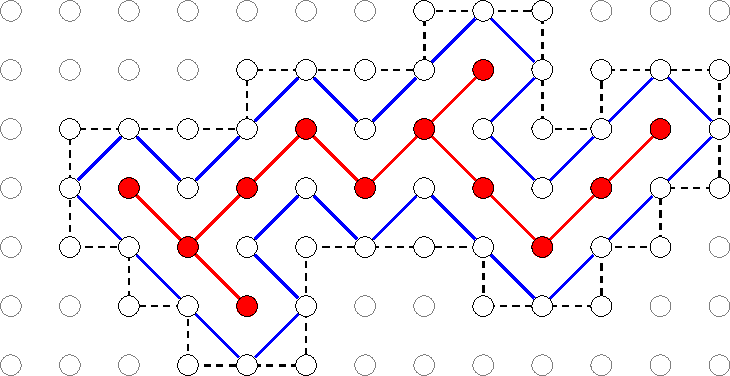
\includegraphics[width=0.5\textwidth]{figures/6/monochromatic.pdf}
\caption{Grid with component $K$ (red), $C_H$ (blue), and $C_G$ (dashed).}
\label{fig:border}
\end{figure} 
